\documentclass{article}
\usepackage{tikz}
\begin{document}

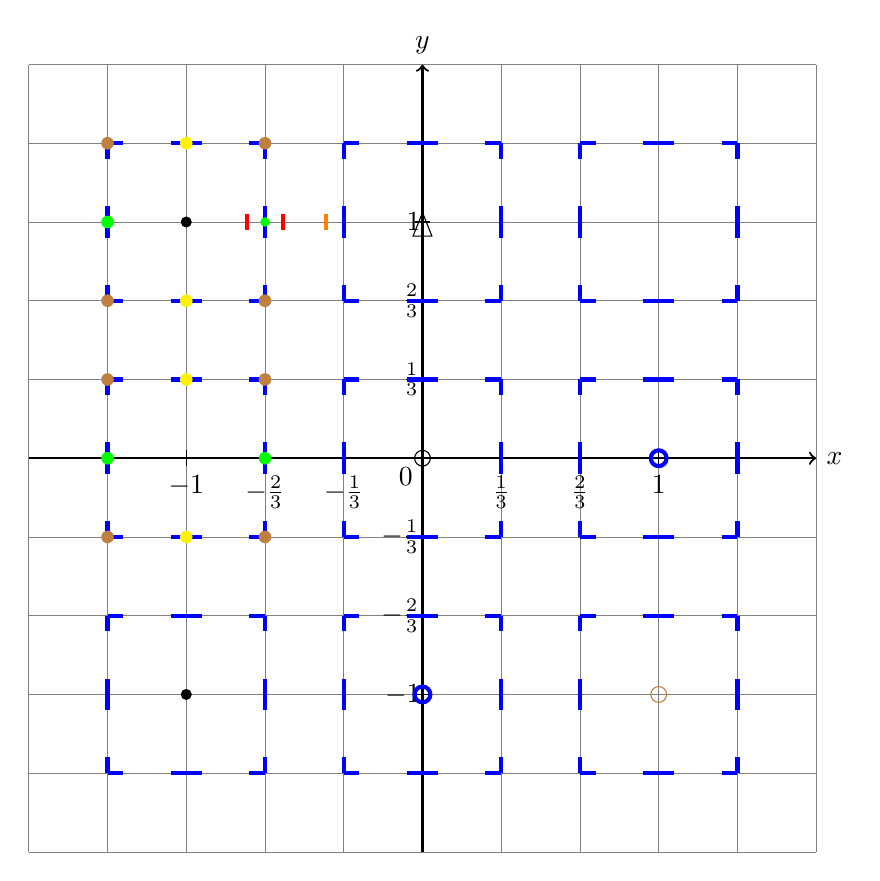
\begin{tikzpicture}[scale=1]
  % Draw grid
  \draw[step=1cm,gray,very thin] (-5,-5) grid (5,5);

  % Draw axes
  \draw[->,thick] (-5,0) -- (5,0) node[right] {$x$};
  \draw[->,thick] (0,-5) -- (0,5) node[above] {$y$};

\draw (-3,0.1) -- (-3,-0.1) node[below] {$-1$};
\draw (-2,0.1) -- (-2,-0.1) node[below] {$-\frac{2}{3}$};
\draw (-1,0.1) -- (-1,-0.1) node[below] {$-\frac{1}{3}$};
\draw (1,0.1) -- (1,-0.1) node[below] {$\frac{1}{3}$};
\draw (2,0.1) -- (2,-0.1) node[below] {$\frac{2}{3}$};
\draw (3,0.1) -- (3,-0.1) node[below] {$1$};
\draw (-0.1, 3) -- (0.1, 3) node [left] {$1$};
\draw (-0.1, 2) -- (0.1, 2) node [left] {$\frac{2}{3}$};
\draw (-0.1, 1) -- (0.1, 1) node [left] {$\frac{1}{3}$};
\draw (-0.1, -1) -- (0.1, -1) node [left] {$-\frac{1}{3}$};
\draw (-0.1, -2) -- (0.1, -2) node [left] {$-\frac{2}{3}$};
\draw (-0.1, -3) -- (0.1, -3) node [left] {$-1$};

  % Origin
  \node[below left] at (0,0) {0};
 % \draw (-0.12,-0.12) -- (0,0.12) -- (0.12,-0.12) -- cycle;
  \draw (-0.12,2.82) -- (0,3.12) -- (0.12,2.82) -- cycle;



  % (-1,0)

  \draw [blue, line width=1.5pt] (-3.2, 1) -- (-2.8, 1); 
  \fill[yellow] (-3,1) circle (0.08cm);


  \draw [blue, line width=1.5pt] (-2.2,1) -- (-2,1);
  \draw [blue, line width=1.5pt](-2, 1) -- (-2, 0.8);
  \fill[brown] (-2,1) circle (0.08cm);

  \draw [blue, line width=1.5pt] (-2, 0.2) -- (-2,-0.2);
  \fill[green] (-2,0) circle (0.08cm);

  \draw [blue, line width=1.5pt] (-2, -0.8) -- (-2, -1);
  \draw [blue, line width=1.5pt] (-2.2, -1) -- (-2,-1);
  \fill[brown] (-2,-1) circle (0.08cm);

  \draw [blue, line width=1.5pt] (-3.2, -1) -- (-2.8, -1);
  \fill[yellow] (-3,-1) circle (0.08cm);

  \draw [blue, line width=1.5pt] (-4,-1) -- (-3.8,-1);
  \draw [blue, line width=1.5pt] (-4, -1) -- (-4, -0.8);
  \fill[brown] (-4,-1) circle (0.08cm);

  \draw [blue, line width=1.5pt] (-4, -0.2) -- (-4, 0.2);
  \fill[green] (-4,0) circle (0.08cm);

  \draw [blue, line width=1.5pt] (-4, 0.8) -- (-4, 1);
  \draw [blue, line width=1.5pt] (-4, 1) -- (-3.8, 1);
  \fill[brown] (-4,1) circle (0.08cm);

  %(0,0)
\draw (0,0) circle (0.1cm);
\draw [blue, line width=1.5pt](-0.2, 1) -- (0.2,1);

\draw [blue, line width=1.5pt] (0.8,1) -- (1,1);
\draw [blue, line width=1.5pt] (1, 1) -- (1, 0.8);

\draw [blue, line width=1.5pt] (1, 0.2) -- (1,-0.2);

\draw [blue, line width=1.5pt] (1, -0.8) -- (1, -1);
\draw [blue, line width=1.5pt] (0.8, -1) -- (1, -1);

\draw [blue, line width=1.5pt] (-0.2, -1) -- (0.2, -1);

\draw [blue, line width=1.5pt] (-1, -1) -- (-0.8, -1);
\draw [blue, line width=1.5pt] (-1, -1) -- (-1, -0.8);

\draw [blue, line width=1.5pt] (-1, -0.2) -- (-1, 0.2);

\draw [blue, line width=1.5pt] (-1, 0.8) -- (-1, 1);
\draw [blue, line width=1.5pt] (-1, 1) -- (-0.8, 1);

%(1,0)
\draw [blue, line width=1.5pt] (3,0) circle (0.1cm);
\draw [blue, line width=1.5pt] (2.8,1) -- (3.2,1);

\draw [blue, line width=1.5pt] (3.8,1) -- (4,1);
\draw [blue, line width=1.5pt] (4, 1) -- (4, 0.8);

\draw [blue, line width=1.5pt] (4, 0.2) -- (4,-0.2);

\draw [blue, line width=1.5pt] (4, -0.8) -- (4, -1);
\draw [blue, line width=1.5pt] (3.8, -1) -- (4, -1);

\draw [blue, line width=1.5pt] (2.8, -1) -- (3.2, -1);

\draw [blue, line width=1.5pt] (2, -1) -- (2.2, -1);
\draw [blue, line width=1.5pt](2, -1) -- (2, -0.8);

\draw [blue, line width=1.5pt](2, -0.2) -- (2, 0.2);

\draw [blue, line width=1.5pt](2, 0.8) -- (2, 1);
\draw [blue, line width=1.5pt](2, 1) -- (2.2, 1);

%(-1,1)
\fill (-3,3) circle (2pt);
\draw [blue, line width=1.5pt](-3.2, 4) -- (-2.8, 4); 
\fill[yellow] (-3,4) circle (0.08cm);

\draw [blue, line width=1.5pt](-2.2, 4) -- (-2, 4);
\draw [blue, line width=1.5pt](-2, 4) -- (-2, 3.8);
\fill[brown] (-2,4) circle (0.08cm);

\draw [blue, line width=1.5pt](-2, 3.2) -- (-2, 2.8);
\fill[green] (-2,3) circle (0.06cm);

%%%%%%%%%%%%%%%%%%%%%%%%%%%%%%%
\draw [red, line width=1.5pt] (-2.23,3.1) -- (-2.23,2.9);
\draw [red, line width=1.5pt] (-1.77,3.1)  -- (-1.77,2.9);
%%%%%%%%%%%%%%%%%%%%%%%%%%%%%%%








\draw [blue, line width=1.5pt](-2, 2.2) -- (-2, 2);
\draw [blue, line width=1.5pt](-2.2, 2) -- (-2, 2);
\fill[brown] (-2,2) circle (0.08cm);

\draw [blue, line width=1.5pt](-3.2, 2) -- (-2.8, 2);
\fill[yellow] (-3,2) circle (0.08cm);

\draw [blue, line width=1.5pt](-4, 2) -- (-3.8, 2);
\draw [blue, line width=1.5pt](-4, 2) -- (-4, 2.2);
\fill[brown] (-4,2) circle (0.08cm);

\draw [blue, line width=1.5pt](-4, 2.8) -- (-4, 3.2);
\fill[green] (-4,3) circle (0.08cm);

\draw [blue, line width=1.5pt](-4, 3.8) -- (-4, 4);
\draw [blue, line width=1.5pt](-4, 4) -- (-3.8, 4);
\fill[brown] (-4,4) circle (0.08cm);

%(-1,-1)
\fill (-3,-3) circle (2pt);
\draw [blue, line width=1.5pt](-3.2, -2) -- (-2.8, -2); 

\draw [blue, line width=1.5pt](-2.2, -2) -- (-2, -2);
\draw [blue, line width=1.5pt](-2, -2) -- (-2, -2.2);

\draw [blue, line width=1.5pt](-2, -2.8) -- (-2, -3.2);

\draw [blue, line width=1.5pt](-2, -3.8) -- (-2, -4);
\draw [blue, line width=1.5pt](-2.2, -4) -- (-2, -4);

\draw [blue, line width=1.5pt](-3.2, -4) -- (-2.8, -4);

\draw [blue, line width=1.5pt](-4, -4) -- (-3.8, -4);
\draw [blue, line width=1.5pt](-4, -4) -- (-4, -3.8);

\draw [blue, line width=1.5pt](-4, -3.2) -- (-4, -2.8);

\draw [blue, line width=1.5pt](-4, -2.2) -- (-4, -2);
\draw [blue, line width=1.5pt](-4, -2) -- (-3.8, -2);

%(1,1)
\draw [blue, line width=1.5pt](2.8,4) -- (3.2,4);

\draw [blue, line width=1.5pt](3.8,4) -- (4,4);
\draw [blue, line width=1.5pt](4, 4) -- (4, 3.8);

\draw [blue, line width=1.5pt](4, 3.2) -- (4, 2.8);

\draw [blue, line width=1.5pt](4, 2.2) -- (4, 2);
\draw [blue, line width=1.5pt](3.8, 2) -- (4, 2);

\draw [blue, line width=1.5pt](2.8, 2) -- (3.2, 2);

\draw [blue, line width=1.5pt](2, 2) -- (2.2, 2);
\draw [blue, line width=1.5pt](2, 2) -- (2, 2.2);

\draw [blue, line width=1.5pt](2, 2.8) -- (2, 3.2);

\draw [blue, line width=1.5pt](2, 3.8) -- (2, 4);
\draw [blue, line width=1.5pt](2, 4) -- (2.2, 4);

%(0,1)
%\draw [blue, line width=1.5pt](0,3) circle (0.1cm);
\draw [blue, line width=1.5pt](-0.2, 4) -- (0.2, 4);

\draw [blue, line width=1.5pt](0.8, 4) -- (1, 4);
\draw [blue, line width=1.5pt](1, 4) -- (1, 3.8);

\draw [blue, line width=1.5pt](1, 3.2) -- (1, 2.8);

\draw [blue, line width=1.5pt](1, 2.2) -- (1, 2);
\draw [blue, line width=1.5pt](0.8, 2) -- (1, 2);

\draw [blue, line width=1.5pt](-0.2, 2) -- (0.2, 2);

\draw [blue, line width=1.5pt](-1, 2) -- (-0.8, 2);
\draw [blue, line width=1.5pt](-1, 2) -- (-1, 2.2);

\draw [blue, line width=1.5pt](-1, 2.8) -- (-1, 3.2);
%%%%%%%%%%%%%%%%%%%%%%%%%%%%%%%

\draw [orange, line width=1.5pt] (-1.23, 3.1) -- (-1.23, 2.9);



%%%%%%%%%%%%%%%%%%%%%%%%%%%%%%%

\draw [blue, line width=1.5pt](-1, 3.8) -- (-1, 4);
\draw [blue, line width=1.5pt](-1, 4) -- (-0.8, 4);

%(0,-1)
\draw [blue, line width=1.5pt](0,-3) circle (0.1cm);
\draw [blue, line width=1.5pt](-0.2, -2) -- (0.2, -2);

\draw [blue, line width=1.5pt](0.8, -2) -- (1, -2);
\draw [blue, line width=1.5pt](1, -2) -- (1, -2.2);

\draw [blue, line width=1.5pt](1, -2.8) -- (1, -3.2);

\draw [blue, line width=1.5pt](1, -3.8) -- (1, -4);
\draw [blue, line width=1.5pt](0.8, -4) -- (1, -4);

\draw [blue, line width=1.5pt](-0.2, -4) -- (0.2, -4);

\draw [blue, line width=1.5pt](-1, -4) -- (-0.8, -4);
\draw [blue, line width=1.5pt](-1, -4) -- (-1, -3.8);

\draw [blue, line width=1.5pt](-1, -3.2) -- (-1, -2.8);

\draw [blue, line width=1.5pt](-1, -2.2) -- (-1, -2);
\draw [blue, line width=1.5pt](-1, -2) -- (-0.8, -2);

%(1,-1)
\draw[brown] (3,-3)circle (0.1cm);
\draw [blue, line width=1.5pt](2.8, -2) -- (3.2, -2);

\draw [blue, line width=1.5pt](3.8, -2) -- (4, -2);
\draw [blue, line width=1.5pt](4, -2) -- (4, -2.2);

\draw [blue, line width=1.5pt](4, -2.8) -- (4, -3.2);

\draw [blue, line width=1.5pt](4, -3.8) -- (4, -4);
\draw [blue, line width=1.5pt](3.8, -4) -- (4, -4);

\draw [blue, line width=1.5pt](2.8, -4) -- (3.2, -4);

\draw [blue, line width=1.5pt](2, -4) -- (2.2, -4);
\draw [blue, line width=1.5pt](2, -4) -- (2, -3.8);

\draw [blue, line width=1.5pt](2, -3.2) -- (2, -2.8);

\draw [blue, line width=1.5pt](2, -2.2) -- (2, -2);
\draw [blue, line width=1.5pt](2, -2) -- (2.2, -2);

\end{tikzpicture}

\end{document}